% !TEX encoding = UTF-8 Unicode
\documentclass[a4paper]{article}

\usepackage{color}
\usepackage{url}
\usepackage[T2A]{fontenc} % enable Cyrillic fonts
\usepackage[utf8]{inputenc} % make weird characters work
\usepackage{graphicx}
\graphicspath{ {./images/} }
\usepackage{amsfonts}
\usepackage[english,serbian]{babel}
%\usepackage[english,serbianc]{babel} %ukljuciti babel sa ovim opcijama, umesto gornjim, ukoliko se koristi cirilica

\usepackage[unicode]{hyperref}
\hypersetup{colorlinks,citecolor=green,filecolor=green,linkcolor=blue,urlcolor=blue}

\usepackage{listings}
\usepackage{mathtools}
\usepackage{dirtytalk}
\usepackage{epigraph}


%\newtheorem{primer}{Пример}[section] %ćirilični primer
\newtheorem{primer}{Primer}[section]

\definecolor{mygreen}{rgb}{0,0.6,0}
\definecolor{mygray}{rgb}{0.5,0.5,0.5}
\definecolor{mymauve}{rgb}{0.58,0,0.82}

\lstset{ 
  backgroundcolor=\color{white},   % choose the background color; you must add \usepackage{color} or \usepackage{xcolor}; should come as last argument
  basicstyle=\scriptsize\ttfamily,        % the size of the fonts that are used for the code
  breakatwhitespace=false,         % sets if automatic breaks should only happen at whitespace
  breaklines=true,                 % sets automatic line breaking
  captionpos=b,                    % sets the caption-position to bottom
  commentstyle=\color{mygreen},    % comment style
  deletekeywords={...},            % if you want to delete keywords from the given language
  escapeinside={\%*}{*)},          % if you want to add LaTeX within your code
  extendedchars=true,              % lets you use non-ASCII characters; for 8-bits encodings only, does not work with UTF-8
  firstnumber=1000,                % start line enumeration with line 1000
  frame=single,	                   % adds a frame around the code
  keepspaces=true,                 % keeps spaces in text, useful for keeping indentation of code (possibly needs columns=flexible)
  keywordstyle=\color{blue},       % keyword style
  language=Python,                 % the language of the code
  morekeywords={*,...},            % if you want to add more keywords to the set
  numbers=left,                    % where to put the line-numbers; possible values are (none, left, right)
  numbersep=5pt,                   % how far the line-numbers are from the code
  numberstyle=\tiny\color{mygray}, % the style that is used for the line-numbers
  rulecolor=\color{black},         % if not set, the frame-color may be changed on line-breaks within not-black text (e.g. comments (green here))
  showspaces=false,                % show spaces everywhere adding particular underscores; it overrides 'showstringspaces'
  showstringspaces=false,          % underline spaces within strings only
  showtabs=false,                  % show tabs within strings adding particular underscores
  stepnumber=2,                    % the step between two line-numbers. If it's 1, each line will be numbered
  stringstyle=\color{mymauve},     % string literal style
  tabsize=2,	                   % sets default tabsize to 2 spaces
  title=\lstname                   % show the filename of files included with \lstinputlisting; also try caption instead of title
}

\begin{document}

\title{Optimizacija rojem čestica\\ \small{Seminarski rad u okviru kursa\\Metodologija stručnog i naučnog rada\\ Matematički fakultet}}

\author{Nevena Soldat, Milena Kurtić, Tijana Živković, Ana Miloradović\protect\\
\small{\texttt{nevenasoldat@gmail.com,}  \texttt{mimikurtic67@gmail.com,}} \\ \small{\texttt{tijanazivkovic6@gmail.com,} \texttt{ana.miloradovic7@gmail.com}}}

%\date{9.~april 2015.}

\maketitle

\abstract{ Kennedy i Eberhart (2001): \\
\say{... gledamo u paradigmu koja je u svom začeću, puna potencijala i novih ideja i novih perspektiva... Istraživači u mnogim zemljama eksperimentišu sa rojevima čestica... Mnoga pitanja koja su postavljena još uvek nisu dobila dobar odgovor.}

U ovom radu opisaćemo osnovni algoritam za optimizaciju rojem čestica, kao i neke od postojećih varijacija. Objasnićemo jednostavnije algoritme sa jedinstvenim rešenjem, ali i neke naprednije. Tema će biti i socijalne strukture na kojima se on zasniva, kao i koje su moguće primene. 
}

\tableofcontents

\newpage

\section{Uvod}
\label{sec:uvod}

Inteligencija rojeva predstavlja jednu od pet glavnih paradigmi Računarske Inteligencije (Computation Intelligence - CI). Jedinke u okviru grupe (roja) dele prikupljene informacije u zajedničkom cilju da reše neki problem, koje se propagiraju kroz celu grupu tako da se problem rešava mnogo efikasnije nego što bi to mogla pojedinačna jedinka.
Prvi i dosta značajan doprinos u polju inteligencije rojeva imao je južnoafrički pesnik Eugene N Marais koji je proučavao socijalno ponašanje kako majmuna, tako i mrava. Posle njega, ranih 1990-ih godina, Marco Dorigo modeluje ponašanje kolonija mrava. Zatim, 1995, Eberhart i Kennedy razvijaju algoritam optimizacije rojem čestica, na osnovu posmatranog jata ptica.
Optimizacija rojem čestica (eng. Particle Swarm Optimization - PSO) je stohastička optmizaciona tehnika zasnovana na veoma inteligentnom kolektivnom ponašanju nekih organizama kao što su insekti, ptice i ribe. Algoritam optimizacije rojem čestica otkriven je sasvim slučajno od strane Eberharta i Kenedija, pri pokušaju da se na računaru simulira kretanje jata ptica. Prvobitna namera bila je da se grafički prikaže nepredvidiva koreografija jata ptica, sa ciljem da se otkriju obrasci koji omogućavaju pticama da lete sinhronizovano, i da zadrže optimalnu formaciju pri naglim promenama pravaca. Sada je cilj kreiranje jednostavnog i efikasnog optimizacionog algoritma. Od kada je prvi put predstavljen 1995. doživeo je niz poboljšanja i nastale su brojne varijacije ovog algoritma. 


\section{Algoritam za optimizaciju rojem čestica}
Kako bismo lakše razumeli algoritam možemo zamisliti roj pčela koje lete preko polja sa cvećem. Roj ima urođenu želju da pronađe poziciju gde je cveće najgušće raspoređeno. Takođe, pčele nemaju nikakvo znanje o polju na kom se nalaze. Tako počinju svoju pretragu u različitim smerovima. Svaka pčela pamti mesta na kojima je bila i na kojim je bilo najviše cveća, i tu informaciju može preneti komunikacijom sa ostatkom roja. Kako vreme prolazi, pčele biraju da li će se vratiti na svoje prethodno pronađene najbolje lokacije ili će ići ka lokacijama koje su dobile od ostalih pčela. One koje oklevaju će ići u oba pravca i nalaziće se negde između ciljanih lokacija, u zavisnosti od toga da li će socijalan uticaj biti dominantan ili ne. Povremeno, pčela može da preleti preko dela polja u kom se nalazi više cveća od do sad otkrivenih lokacija. Tada će se čitav roj povlačiti ka novootkrivenoj lokaciji.
\begin{figure}[htp]
    \centering
    \includegraphics[scale=1.2]{bees.png}
    \caption{Prikaz PSO algoritma na kojem pčele traže cveće}
    \label{fig:bees}
\end{figure}
\\ \indent Na slici 1, isprekidane linije predstavljaju zamišljene putanje pčela, a strelice prikazuju dve komponente brzine (lokalno najbolju poziciju i globalno najbolju poziciju). Pčela u gornjem delu slike je pronašla globalno najbolju poziciju, dok je pčela sa leve strane pronašla lokalno najbolju poziciju. Pčela u donjem delu slike prikazuje da iako nije pronašla lokalno najbolju poziciju, ide ka globalno najboljoj poziciji. \\
\indent Na ovaj način pčele pretražuju polje tako što menjaju brzine i pravac kretanja u zavisnosti od toga da li je imala uspeha da pronađe cveće u odnosu na čitav roj. Takođe pčele znaju da izbegavaju mesta koja nisu imala puno cveća. Na kraju će pretražiti celo polje, i nalaziće se iznad mesta na kojem je najveća gustina cveća.

\subsection{Originalni PSO}
Algoritam za optimizaciju rojem čestica sadrži jedinke (čestice) koje se se kreću kroz višedimenzioni prostor pretrage, a pozicije jedinki se menjaju u skladu sa sopstvenim iskustvom, kao i sa iskustvom susednih jedinki. Svaka od tih čestica predstavlja jedno moguće rešenje.
Neka je $x_i(t)$ pozicija čestice \textit{i} u prostoru pretrage u trenutku \textit{t}. Pozicija čestice se menja dodavanjem brzine, $v_i(t)$ na trenutnu poziciju. \[x_i(t+1) = x_i(t) + v_i(t+1) \]
Njihovo kretanje se usmerava imajući u vidu njihovu trenutnu poziciju, njihovu do sada najbolju poziciju, kao i do sada najbolju poziciju čitavog roja. Kognitivna komponenta algoritma predstavlja tendenciju vraćanja u lično najbolje rešenje, dok socijalna komponenta predstavlja tendenciju ka globalno najboljem rešenju. Brzina se računa kao: \[ v_i(t+1) = v_i(t) + c_1r_1(p_i(t) - x_i(t)) + c_2r_2(p_g(t) - x_i(t))\]
gde $p_i(t)$ predstavlja najbolju do sada poziciju čestice \textit{i} u trenutku t, dok je $p_g(t)$ globalno najbolje rešenje (pozicija) do trenutka t. Parametri $r_1$ i $r_2$ su nasumične vrednosti izabrane iz uniformne raspodele na intervalu [0,1], dok su parametri $c_1$ i $c_2$ konstante koje predstavljaju pozitivna ubrzanja čija je uloga da skaliraju značaj kognitivne, odnosno socijalne komponente brzine. 
Pseudokod originalnog PSO algoritma: \\ \\
\textbf{Algoritam} \textit{osnovni} PSO: \\ 
Kreiraj i inicijalizuj $n_s$ - dimenzioni roj;\\
\textbf{ponavljaj} \\ 
\hspace*{5mm}\textbf{za} \textit{svaku česticu} $\textit{i} = 1,...,n_s$ \textbf{uradi} \\
\hspace*{5mm} // postavi lokalno najbolju poziciju \\
\hspace*{10mm} \textbf{ako} $f(x_i) < f(p_i)$ \textbf{onda} \\
\hspace*{15mm} $p_i = x_i;$ \\
\hspace*{10mm} \textbf{kraj} \\
\hspace*{5mm}//postavi globalno najbolju poziciju \\\
\hspace*{10mm}\textbf{ako} $f(p_i) < f(p_g)$ \textbf{onda} \\
\hspace*{15mm} $p_g = p_i;$ \\
\hspace*{10mm} \textbf{kraj} \\
\hspace*{5mm} \textbf{kraj} \\
\hspace*{5mm} \textbf{za} \textit{svaku česticu} $i = 1,...,n_s$ \textbf{uradi}\\
\hspace*{10mm} ažuriraj brzinu; \\
\hspace*{10mm} ažiriraj poziciju; \\
\hspace*{5mm} \textbf{kraj} \\
\textbf{dok} nije ispunjen zahtev za zaustavljanje; \\ \\Funkcija $f:\mathbb{R}^{n_x} \to \mathbb{R}$ je fitnes funkcija. Fitnes funkcija računa koliko je dobijeno rešenje blisko optimalnom, odnosno meri kvalitet rešenja.
\subsection{Komponente brzine PSO algoritma}
Brzina \textit{i}-te čestice ima tri komponente:\\
\begin{itemize}
    \item \textbf{Prethodna vrednost brzine}, $\textbf{v}_i(t)$, koja čuva prethodni pravac kretanja čestice. Može se reći da je ona moment koji sprečava česticu da drastično promeni pravac. 
    \item \textbf{Kognitivna komponenta}, $c_1\textbf{r}_1(\textbf{p}_i - \textbf{x}_i)$, koja meri rezultat čestice \textit{i} u ondosu na prethodne. Može se opisati kao pamćenje najbolje pozicije u kojoj se čestica do sada našla. Efekat ove komponente je tendencija čestica da se vrate na pronadjene najbolje pozicije. Kennedy i Eberhart su nazivali koginitivnu komponentu \say{nostalgija} čestice.
    \item \textbf{Socijalna komponenta}, $c_2\textbf{r}_2(\textbf{p}_g - \textbf{x}_i)$, koja meri rezultat čestice \textit{i} u odnosu na sve susedne čestice. Efekat ove komponente je tendencija čestice da se kreće ka najboljoj poziciji pronađenoj od strane susednih čestica.
\end{itemize}

\begin{figure}[htp]
    \centering
    \includegraphics[scale=1.7]{velocity.png}
    \caption{Prikaz promene brzine}
    \label{fig:velocity}
\end{figure}


\subsection{Algoritmi gbest i lbest PSO}
\label{subsec:podnaslov1}

U slučaju globalno najboljeg PSO algoritma (\textit{gbest}), susedi za svaku česticu su zapravo čitav roj. On implementira topologiju zvezde. U topologiji zvezde socijalna komponenta brzine čestice predstavlja informaciju dobijenu od svih čestica u roju. 

Lokalno najbolji PSO (\textit{lbest}) koristi topologiju prstena, gde svaka čestica ima određeni broj suseda. Socijalna komponenta predstavlja informaciju koju razmenjuju susedi čestice. Doprinos jedinke brzini je proporcionalna razdaljini između čestice i najbolje pozicije koju su pronašli susedi. 

Važno je napomenuti da kod osnovnog PSO algoritma čestice nisu povezane. Razvijene su mnoge strategije na osnovu kojih se bira susedstvo, kao što je razdaljina u prostoru. Međutim, preferirano rešenje je odabir na osnovu indeksa, i za to postoje dva glavna razloga:
\begin{enumerate}
    \item Za pristupe koji podrazumevaju računanje udaljenosti između čestica, potrebno je naći Euklidsko rastojanje svih parova čestica, a to ima veliku složenost ($(n_s)^2$).
    \item Lakše je prosleđivanje informacije o dobrim rešenjima svim česticama, nezavisno od njihove lokacije u prostoru pretrage.
    
\end{enumerate}

\subsubsection{Poređenje gbest i lbest PSO algoritma}
Dve verzije PSO algoritma koje smo opisali su slične u smislu da obe teže ka globalno najboljem rešenju. Međutim postoje dve osnovne razlike:
\begin{itemize}
    \item Zbog bolje povezanosti čestica u gbest algoritmu, on brže konvergira ka rešenju. Cena brže konvergencije je manja raznovrsnost.
    \item Kao posledica veće raznovrsnosti (što podrazumeva da je veći deo prostora pretrage pokriven), lbest PSO ima manje šanse da ostane zaroboljen u lokalnom optimumu. U većini slučajeva, topologija prstena kao kod lbest PSO algoritma poboljšava rezultate.
\end{itemize}

\section{Osnovne varijacije}
Postoji nekoliko modifikacija osnovnog PSO algoritma \cite{rini2011particle}, a one su razvijane da bi poboljšale brzinu konvergencije i kvalitet rešenja koji ovaj algoritam nalazi.

\subsection{Smanjenje brzina}
Za efikasnost i tačnost algoritma optimizacije važno je napraviti balans između eksploracije i eksploatacije. 
$Eksploracija$ se odnosi na sposobnost algoritma pretrage da istražuje različite regione prostora pretrage da bi se pronašao dobar optimum, dok je $eksploatacija$ sposobnost  da se pretraga koncentriše oko regije koje garantuje nalaženje rešenja da bi se poboljšao kandidat rešenja. Ovo su konktradiktorni ciljevi koje treba dovesti u balans radi dobijanja dobrog optimizacionog algoritma.

Ažuriranja brzina u gorenavedenoj jednačini, predstavljena trima uslovima, doprinose veličini koraka čestice. U ranijim, osnovnim PSO algoritmima je primećeno da brzina brzo dostiže velike vrednosti, specijalno kod čestica koje su daleko od najboljih u okruženju i najboljih sopstvenih pozicija. Tim čestim ažuriranjima položaja jedinke polako napuštaju granice prostora pretrage, tj. divergiraju, pa se te brzine smanjuju da bi čestice ostale u okviru granica. Ako brzina prelazi maksimalnu brzinu, postavlja se na taj maksimalnu brzinu, inace se brzina na standardni način ažurira.

\begin{equation}
    v_{ij}(t+1) = \begin{cases}
                
            v'_{ij}(t+1)  & if  v'_{ij}(t+1) < V_{max,j}\\
            V_{max,j}  & if  v'_{ij}(t+1) \geq V_{max,j}
           
             \end{cases}
\end{equation}

Velike vrednosti maksimalne brzine olakšavaju istraživanje na globalnom nivou, dok manje vrednosti podstiču lokalnu eksploataciju. I premale i prevelike vrednosti maksimalne brzine imaju svoje mane. Dok veoma male vrednosti mogu da povećaju broj vremenskih koraka do nalaženja optimalne vrednosti, tako veoma velike vrednosti brzina mogu dovesti da se sasvim propusti dobar region, ali se uz to čestice ipak brže kreću. 
Tako osim prblema balansa eksploracije i eksploatacije treba pronaći i dobar balans za svaki $V_{max}$, da ne bude ni premala, a ni prevelika vrednost. Obično se biraju da budu deo domena svake dimenzije prostora pretrage. 

\[V_{max,j} = \delta(x_{max,j} − x_{min,j} ),\]
gde su $x_{max,j}$ i $x_{min,j}$ maksimualne i minimalne vrednosti domena $x$ u dimenziji $j$, a $\delta \in (0, 1]$.
Vrednosti $\delta$ zavisi od samog problema.

Postoje i mane, promene brzine ne menjaju samo veličinu koraka, već i pravac u kome će se čestica kretati, to može biti prednost-omogućava bolju eksploraciju, ali isto tako može da dovede do toga da optimum uopšte ne bude pronađen.

\begin{figure}[htp]
    \centering
    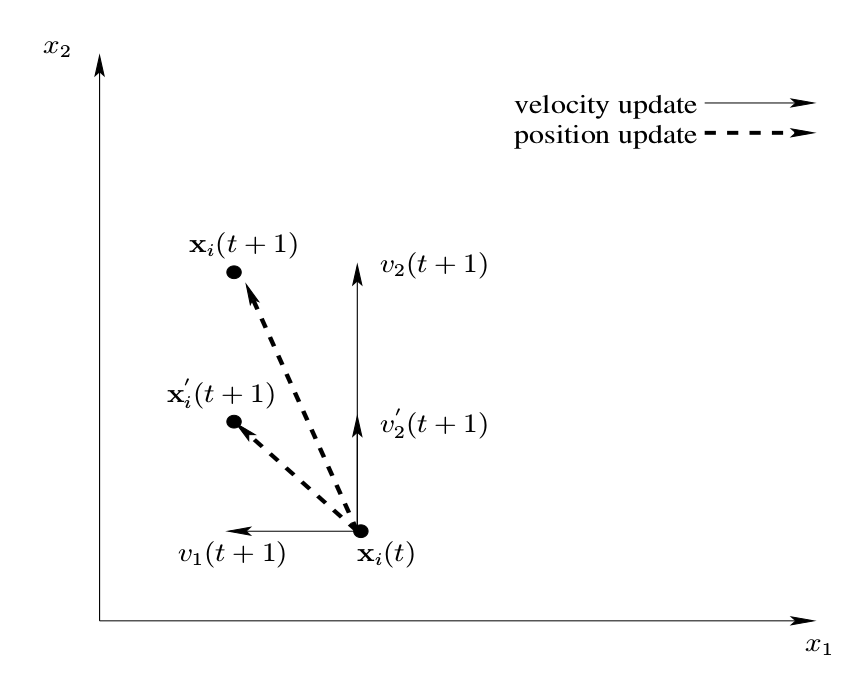
\includegraphics[scale=0.3]{slika3_1.png}
    \caption{Efekat smanjenja brzine}
    \label{fig:velocity}
\end{figure}

Postoji još i problem kada su sve vrednosti jednake $V_{max}$, a ako se ne preduzme ništa povodnom toga, čestice se zaglavljuju unutar ograničene oblasti $[x_i(t)-V_{max} , x_i(t) + V_{max} ]$.  Ovaj problem se može rešiti uvođenjem inercijske težine ili smanjivanjem  $V_{max}$ vrednosti vremenom, tako što pretraga počine s velikim vrednostima i tako se pretražuje prostor, a zatim se postepeno smanjuje. Tako se ograničava globalna pretraga i osvrće se na lokalnu u već kasnim fazama pretraživanja. $V_{max}$ se može menjati kada nema napretka u globalno najboljoj poziciji u toku određenog broja uzastopnih iteracija, ili se može eksponencijalno smanjivati.

\subsection{Inercijalna težina}
Ovaj pristup balansa izmedju eksploracije i eksploatacije nastao je da bi se eliminisalo koriščenje smanjenje brzina. Težina $w$  kontroliše koliko će prethodni pravac leta uticati na novu brzinu. Sada jednačina izgleda ovako:

\[v_{ij}(t+1) = wv_{ij}(t) + c_1r_{1j}(t)[y_{ij}(t) - x_{ij}(t)] + c_2r_{2j}(t)[\hat{y}_{ij}(t) - x_{ij}(t)] \]

Dolazi do promene jednačine ažuriranja brzina kod $gbest$ i $lbest$ PSO algoritama.
Kod ovog pristupa je vrednost $w$ izuzetno važna za ostvarivanje konvergencije, kao i za prethodno pomenuti balans između eksploracije i ekspoatacije. Razlikuju se slučaji kada je $w ≥ 1$, tada se brzine povećavaju tokom vremena prema Vmax i roj divergira, dok za $w < 0$ brzine opadaju sve dok ne dostignu nulu i time se algoritam zaustavlja, a za $0 < w < 1$ čestice usporavaju, pa konvergencija zavisi od vrednosti $c_1$ i $c_2$. Tako velike vrednosti  $w$ olakšavaju eksploraciju, dok male vrednosti podstiče loakalnu eksploataciju. 
Kao i kod $V_{max}$, i ovaj pristup zavisi od samog problema. U početku se koristila konstantna vrednost $w$, za svaku česticu u svakoj dimenziji, a kasnije se započelo sa dinamičkim promenama vrednosti, počinjavši od velike inercijske vrednosti koja se vremenom smanjivala. Time se u početnim koracima dozvoljava da čestice istražuju, a zatim počinju da favorizuju određene delove područja kako vreme odmiče.
Vrednost $w$ se mora birati zajedno sa vrednostima $c_1$ i $c_2$ (konstante ubrzanja). $$w > \frac{1}{2}(c_1 + c_2) - 1$$ Ovo garantuje da će putanje čestica voditi ka konvergenciji, a ukoliko ovaj uslov nije zaodovoljen, može doći do cikličnog ponašanja, ili pak divergencije.

\subsection{Koeficijent suženja}
Clerc je razvio pristup sličan inerciji težina, gde su brzine ograničene konstantom \chi koji se naziva koeficijentom suženja. Jednačina sada izgleda ovako:

\[v_{ij} (t + 1) = \chi[v_{ij} (t) + \phi_1 (y_{ij} (t) - x_{ij} (t)) + \phi_2 (\hat{y}_j (t) - x_{ij} (t))]\]
gde je $$\chi = \frac{2k}{|2-\phi-\sqrt{\phi(\phi-4)}|},$$sa $\phi = \phi_1 +  \phi_2 , \phi_1 = c_1r_1$ i $\phi_2 = c_2r_2$.
Jednačina se primenjuje pod ograničenjima gde je $\phi \geq 4$ i $k$ $\in [0, 1]$
Ovaj pristup napravljen je kao prirodan, dinamički način da se osigura konvergencija ka stabilnoj tački, bez potrebe za smanjivanjem brzine, roj će konvergirati zbog gorenavedenih ograničenja.
Parametar $k$ u jednačini kontroliše sposobnost eksploracije i eksploatacije, za $κ ≈ 0$ se postiže brza konvergencija uz lokalnu eksploataciju, dok za  $κ ≈ 1$ sporo konvergira, sa visokim stepenom eksploracije. $k$ se obično postavlja na konstantnu vrednost.

Razlika između pristupa smanjenja brzina i koeficijenta suženja je ta da smanjenje brzina nije neophodno za model suženja (Eberhart i Shi su pokazali da ako se koriste zajedno mogu da dovedu do brže konvergencije). Model suženja garantuje konvergenciju pod datim ograničenjima i kod njega svaka promena smera čestica mora se izvršiti preko konstnti $\phi_1$ i $\phi_2$.

\subsection{Modeli brzina}
Modeli se razlikuju u komponentama koje su uključene u jednačinu brzine i u tome kako se utvrđuju najbolji položaji. Neki od njih su:
\begin{itemize}
    \item \textbf{Cognition-Only}, kognitivni model isključuje socijalnu komponentu iz jednačine, pa jednačina izgleda ovako: $$v_{ij} (t + 1) = v_{ij} (t) + c_1r_{1j} (t)(y_{ij} (t) - x_{ij} (t)).$$ Ovaj model se može uporediti sa nostalgijom i ilustruje stohastičku tendenciju  da se čestice vraćaju u svoju najbolju poziciju. Ovaj model je sporiji, potrebno je više iteracija da bi se dostiglo dobro rešenje, a, takođe, ne uspeva kada je malo smanjenje brzina i koeficijent ubrzanja.
    \item \textbf{Social-Only}, socijalni model isključuje kognitivnu komponentu iz jednačine: $v_{ij} (t + 1) = v_{ij} (t) + c_2r_{2j} (t)(\hat{y}_j (t) - x_{ij} (t))$ u $gbest$ PSO algoritmu. Kod ovog modela čestice nemaju tendenciju da se vraćaju na prethodno najbolje pozicije, već sve čestice idu ka najboljem položaju svog okruženja. Ovaj model se pokazao bržim od originalnog i kognitivnog modela.
    \item \textbf{Selfless}, kod ovog modela koji je sličan socijalnom, najbolje rešenje iz okruženja se bira isključivo iz suseda čestica. On se pokazao kao brži od socijalnog modela u čak nekoliko problema.
\end{itemize}
\section{Topologije uticaja}

\addcontentsline{toc}{section}{Literatura}
\appendix
\bibliography{bibliografija.bib} 
\bibliographystyle{plain}


\end{document}
